\documentclass[a4paper, 11pt, twoside]{article}
%Petr - pouzivam

%obecne
\usepackage[czech]{babel}
\usepackage[utf8]{inputenc}
%\usepackage[IL2]{fontenc}
\usepackage[T1]{fontenc}
% \usepackage{charter}



\usepackage{xspace}
\usepackage{framed}
\usepackage{mathtools}
\usepackage{pdflscape}
\usepackage[top=3cm, left=3.5cm, right=2.5cm, bottom=3cm, headheight=15pt, includeheadfoot]{geometry}%rozměry stránky
\usepackage{textcomp}
\usepackage{natbib}
\usepackage{hyperref}
\hypersetup{
    bookmarks=true,         % show bookmarks bar?
    unicode=false,          % non-Latin characters in Acrobat’s bookmarks
    pdftoolbar=true,        % show Acrobat’s toolbar?
    pdfmenubar=true,        % show Acrobat’s menu?
    pdffitwindow=false,     % window fit to page when opened
    pdfstartview={FitH},    % fits the width of the page to the window
    pdftitle={Smoderp manual},    % title
    pdfauthor={Kavka ...},     % author
    pdfsubject={Subject},   % subject of the document
    pdfcreator={Creator},   % creator of the document
    pdfproducer={Producer}, % producer of the document
    pdfkeywords={keyword1, key2, key3}, % list of keywords
    pdfnewwindow=true,      % links in new PDF window
    colorlinks=false,       % false: boxed links; true: colored links
    linkcolor=red,          % color of internal links (change box color with linkbordercolor)
    citecolor=green,        % color of links to bibliography
    filecolor=magenta,      % color of file links
    urlcolor=cyan           % color of external links
}
\usepackage[printonlyused]{acronym} %rejstik
% \usepackage{acronym} %rejstik
\makeatletter
\AtBeginDocument{%
  \renewcommand*{\AC@hyperlink}[2]{#2}%
}
\makeatother



%text
\usepackage{subcaption}
\usepackage{listings} % inserting code 
\lstset
{ %Formatting for code in appendix
    language=Python,
    basicstyle=\footnotesize,
%     numbers=left,
%     stepnumber=1,
%     showstringspaces=false,
%     tabsize=1,
%     breaklines=true,
%     breakatwhitespace=true,
}


%tabulky
\usepackage{array}
\usepackage{tabulary}
\usepackage{multirow}
\usepackage{multicol}

%obrazky





% nuti obrazky aby nepretekali do dalsi sekce
\usepackage[section]{placeins}








%Lenka - nepouzivam
\usepackage{longtable}
\usepackage{siunitx}
\usepackage{rotating}
\usepackage[table,xcdraw]{xcolor}
\usepackage{booktabs}
\usepackage{url}
%\usepackage[pdftex,unicode,bookmarksnumbered,raiselinks=true]{hyperref}
% \usepackage{indentfirst}
\usepackage{fancyhdr}
\usepackage[font={footnotesize},labelfont=bf,justification=justified]{caption}
\usepackage{hhline}
\usepackage{colortbl}
\usepackage{array,graphicx}
\usepackage{placeins}

\usepackage{titlesec}



% \usepackage[table]{xcolor}
\usepackage{setspace}


% vetsi mezera mezi odstavci
\setlength{\parskip}{0.5em}


% nadefinovane tvary do flow chart diagramu
% ten jeden po postaven v ./graph/CZflowch
\usepackage{tikz}
\usetikzlibrary{shapes.geometric, arrows}
\tikzstyle{startstop} = [rectangle, rounded corners, minimum width=3cm, minimum height=1cm,text centered, draw=black, fill=red!30]
\tikzstyle{io} = [trapezium, trapezium left angle=70, trapezium right angle=110, minimum width=1cm, minimum height=1cm, text centered, draw=black, fill=blue!30]
\tikzstyle{arrow} = [thick,->,>=stealth]
\tikzstyle{decision} =  [diamond, minimum width=1cm, minimum height=1cm, text centered, text width=2cm, draw=black, fill=green!30, aspect=2]
\tikzstyle{process} = [rectangle, minimum width=3cm, minimum height=1cm, text centered, text width=3cm, draw=black, fill=orange!30]
\tikzstyle{guide} = [inner sep=0pt,minimum size=0mm]
\tikzstyle{line} = [thick]



\usepackage{dirtree}
\usepackage{forest}    % na dir tree ale obecnejsi uziti
% \usepackage{indentfirst}

% tohle je jen prikaz na delatni popisu rovnic 
% jeho pouziti he v kapitole pouzite vztahy treba
\newcommand{\jj}[2]{
   & \acs{#1} & je \acl{#1}#2 \\
}




% kolek okolo cisla, pouzito v tabulce popisujici toolbox
\newcommand*\circled[1]{\tikz[baseline=(char.base)]{
            \node[shape=circle,draw,inner sep=2pt] (char) {{\scriptsize\sffamily#1}};}}



% Název smodepu 
% 
\newcommand{\smod}{SMODERP2D\xspace}


% upraveni casti
\titleformat
{\part} % command
[display] % shape
{\bfseries\Huge} % format
{Část \ \thepart} % label
{5ex} % sep
{
%     \rule{\textwidth}{1pt}
%     \vspace{1ex}
%     \centering
} % before-code
[
\vspace{-2.5ex}%
\rule{\textwidth}{0.3pt}
] % after-code
 
 
%%%% upraveni sekce
% \titlespacing*{\section}
% {0pt}{7.5ex}{2.5ex} 
 

%%%%%%%%%%%%   DĚLENÍ SLOV   %%%%%%%%%%%%%
\hyphenation{bio-logic-kých makro-fyta meteo-stanici geo-engi-nee-ring strmější}
%\DeclareUrlCommand\url{\def\UrlLeft{<}\def\UrlRight{>} \urlstyle{tt}}
\pagestyle{headings}
\setlength{\parskip}{8pt}
\setlength{\parindent}{16pt}

% ridke radkovani
\sloppy

% cesta k obrazkum
\graphicspath{ {img/} {graph/}}

% definice rotace bunky
\newcommand*\rot{\rotatebox[origin=c]{90}}

%http://tex.stackexchange.com/questions/63390/how-to-decrease-spacing-before-chapter-title
\makeatletter
\def\@makechapterhead#1{\vspace*{5\p@}
  {\parindent \z@ \raggedright \normalfont
    \ifnum \c@secnumdepth >\m@ne
        \huge\bfseries \@chapapp\space \thechapter
        \par\nobreak
        \vskip 20\p@
    \fi
    \interlinepenalty\@M
    \Huge \bfseries #1\par\nobreak
    \vskip 40\p@
  }}
\def\@makeschapterhead#1{%
  %%%%%\vspace*{50\p@}% %%% removed!
  {\parindent \z@ \raggedright
    \normalfont
    \interlinepenalty\@M
    \Huge \bfseries  #1\par\nobreak
    \vskip 40\p@
  }}
\makeatother

%http://tex.stackexchange.com/questions/53338/reducing-spacing-after-headings
\titlespacing\section{0pt}{12pt plus 4pt minus 2pt}{12pt plus 2pt minus 2pt}
\titlespacing\subsection{0pt}{12pt plus 2pt minus 2pt}{12pt plus 2pt minus 2pt}
\titlespacing\subsubsection{0pt}{6pt plus 4pt minus 2pt}{6pt plus 2pt minus 2pt}

%definice barev
\definecolor{tab_bg}{HTML}{C0C0C0}
\definecolor{tab_bg_light}{HTML}{EFEFEF}
\definecolor{tab_line}{HTML}{000000}
 
\begin{document}

\title{SMODERP - uživatelská příručka}
\author{Kavka}


% titulni strana bez cisla strany
\clearpage\maketitle
\thispagestyle{empty}



\newpage
\pagenumbering{roman}\setcounter{page}{1} % obsah a seznamy skratek, obrazku a tabulek rimska cislice od i
\tableofcontents\addcontentsline{toc}{section}{Obsah}


%\newpage
%\section*{Seznam zkratek}\addcontentsline{toc}{subsection}{Seznam zkratek}
%\begin{acronym}
\setlength{\parskip}{0ex}
\setlength{\itemsep}{1ex}

\acro{a}[$a$]{parametr MKWA}
\acro{A}[$A$]{průtočná plocha  [$m^{2}$]}
\acro{b}[$b$]{parametr MKWA}
\acro{bhs}[$b$]{šířka dna příčného profilu hydrografické sítě [$m$]}
\acro{brill}[$b_{rill}$]{šířka rýhy [$m$]}
\acro{BrutoSR}[$B_{\Delta t}$]{srážka [$m$]}

\acro{CFL}[$CFL$]{Courant-Friedrich-Lewy podmínka}


\acro{D8}[$D8$]{jednosměrný odtokový algoritmus}

\acro{dT}[$\Delta t$]{časový krok [$s$]}
\acro{dTmax}[$\Delta t_{max}$]{maximální časový krok [$s$]}
\acro{dTmult}[$\Delta t_{mult}$]{multiplikátor časový krok [$-$]}
\acro{dX}[$\Delta x$]{prostorový krok [$m$]}
\acro{dS}[$\frac{\mathrm{d}S}{\mathrm{d}t}$]{změna zásoby [$m^3/s$]}

\acro{ES}[$ES$]{efektivní srážka [$m^3/s$]}
\acro{es}[$es$]{intenzita efektivní srážky [$m/s$]}
\acro{effVrst}[$l_{eff}$]{efektivní vrstevnice [$m$]}

\acro{hcrit}[$h_{crit}$]{kritická hloubka [$m$]}
\acro{hrill}[$h^{rill}$]{hloubka rýhy [$m$]}
\acro{hsur}[$h^{sur}$]{výška hladiny na povrchu [$m$]}
\acro{HyVod}[$k$]{nasycená hydraulická vodivost [$m s^{-1}$]}
\acro{i}[$i$]{řešený element}

\acro{Inf}[$Inf$]{infiltrované množství [$m^3/s$]}
\acro{inf}[$inf$]{intenzita infiltrace [$m/s$]}

% \acro{VItot}[$\dot{I_{tot}}$]{celkový přítok [$m^3/s$]}
\acro{Itot}[$I_{tot}$]{celkový přítok za čas [$m^3/s$]}

\acro{I}[$I$]{sklon [$-$]}

\acro{K}[$K$]{součinitel šířky (pro plošný odtok K = 1)}
\acro{Ki}[$K_i$]{nasycená hydraulická vodivost v buňce $i$ [$m/s$]}

\acro{Lai}[$I_{LAI}$]{poměrná plocha listová}
\acro{lrill}[$l_{rill}$]{délka rýhy [$m$]}
\acro{MKWA}[$MKWA$]{modifikovaná rovnice kinematické vlny}

\acro{mfda}[$mfda$]{vícesměrný odtokový algoritmus}
\acro{m}[$m$]{poměr sklonu svahů (pro obdélník je roven nule)}

\acro{n}[$n$]{mannigův součinitel drsnosti}
\acro{NetoSR}[$I_{N}$]{efektivní srážka}

\acro{PS}[$PS$]{potenciální srážka [$m$]}

% \acro{VOtot}[$\dot{O_{tot}}$]{odtokové množství [$m^{3}$]}
\acro{Otot}[$O_{tot}$]{odtokové množství za čas [$m^{3}/s$]}
% \acro{VOin}[$\dot{O^{in}}$]{objem přítoku ze sousední buňky [$m^{3}$]}
\acro{Oin}[$O^{in}$]{přítok ze sousední buňky  za čas [$m^{3}/s$]}
\acro{oin}[$o^{in}$]{výška vtoku za čas [$m/s$]}
\acro{oinrill}[$o^{in}_{rill}$]{výška vtoku v rýze za čas [$m/s$]}
% \acro{VOout}[$\dot{O^{out}}$]{objem odtoku z buňky [$m^{3}$]}
\acro{Oout}[$O^{out}$]{odtok z buňky  za čas [$m^{3}/s$]}
\acro{oout}[$o^{out}$]{výška odtoku z buňky  za čas [$m/s$]}
\acro{ooutrill}[$o^{out}_{rill}$]{výška odtoku v rýze za čas [$m/s$]}


\acro{Q365}[$Q365$]{základní průtok [$m^3/s$]}

\acro{Orill}[$O_{rill}$]{objem odtoku - rýhový odtok [$m^{3}$]}
\acro{Osur}[$O_{sur}$]{objem odtoku - plošný odtok [$m^{3}$]}
\acro{O}[$O$]{omočený obvod [$m$]}
\acro{PotI}[$I_{POT}$]{potencionální intercepce}
\acro{q}[$q$]{průtok [$m^{3}{s}^{-1}$]}
\acro{qrill}[$q_{rill}$]{průtok v rýhách [$m^{3}/s$]}
\acro{qsur}[$q_{sur}$]{specifický plošný průtok [$m^{2}/s$]}
% \acro{Qtot}[$q_{t}$]{celkový odtok}

\acro{qstream}[$q_{stream}$]{průtok v otevřeném korytě [$m^{3}/s$]}

\acro{Rrill}[$R_{rill}$]{hydraulický poloměr v rýze [m]}
\acro{Rstream}[$R_{stream}$]{hydraulický poloměr v otevřeném korytě [m]}

\acro{ret}[$ret$]{povrchová retence [m]}

\acro{R2}[$R^2$]{koeficient determinace}
\acro{ro}[$\rho$]{hustota [$kg/m^{3}$]}
\acro{rratio}[$rill_{ratio}$]{parametr tvaru rýhy [-]}
\acro{ratio}[$ratio$]{celočíselný faktor dělící časový krok při výpočtu rýhového odtoku}
\acro{slope}[$i_{0}$]{sklon[-]}
\acro{Sorb}[$S$]{sorptivita půdy [$m \sqrt{s}$]}
\acro{Sorbi}[$S_{i}$]{sorptivita půdy  v buňce $i$  [$m \sqrt{s}$]}
\acro{S}[$S$]{sorptivita půdy [$m \sqrt{s}$]}
\acro{t}[$t$]{časový krok[$s$]}
\acro{tausur}[$\tau_{sur}$]{tečné napětí [$Pa$]}
\acro{taucrit}[$\tau_{crit}$]{kritické tečné napětí [$Pa$]}

\acro{Vout}[$V_{out}$]{objem objem odtelkého [$m^{3}$]}

\acro{Vcrit}[$V_{crit}$]{objem vody do kritické hladiny [$m^{3}$]}
\acro{vrill}[$v_{rill}$]{rychlost proudění - rýhový odtok [$m/s$]}
\acro{Vrill}[$V_{rill}$]{objem vody v rýze v daném elementu [$m^{3}$]}
\acro{vsur}[$v_{sur}$]{rychlost proudění - plošný odtok [$m/s$]}
\acro{Vtot}[$V_{tot}$]{celkový objem vody v elementu [$m^{3}$]}
\acro{vstream}[$v_{stream}$]{rychlost proudění v úseku hydrografické sítě [$m/s$]}
\acro{vcrit}[$v_{crit}$]{kritická nevymílací rychlost [$m/s$]}
\acro{X}[$X$]{parametr MKWA}
\acro{Y}[$Y$]{parametr MKWA}
\acro{GIS}[$GIS$]{geografické informační systémy}
\acro{g}[$g$]{gravitační zrychlení [$m/s^{2}$]}

\acro{ij}[$i, j$]{souřadnice elementu - buňky}
\acro{MD8}[$MD8$]{Multiple Flow Direction Algorithm}

\acro{bunka}[$P$]{plocha buňky [$m^2$]}



\end{acronym}
%1to je \ac{MLS}
%2to je \acl{MLS}
%3to je \acs{MLS} 


%\listoffigures\addcontentsline{toc}{subsection}{Seznam obrázků}
%\listoftables\addcontentsline{toc}{subsection}{Seznam tabulek}


\newpage
\pagenumbering{arabic}\setcounter{page}{1}% od uvodu do konce arabske cislice od 1
\section*{Úvod}\addcontentsline{toc}{section}{Úvod}

%!TEX ROOT = ../main.tex


%\clearpage
%\newpage\null\thispagestyle{empty}\newpage

Dostává se Vám do ruky uživatelský manuál modelu \smod. Celý názvem modelu je: Simulační Model Povrchového Odtoku a Erozního Procesu. Tento model lze využít pro výpočet hydrologicko erozních procesů na jednotlivých pozemcích nebo na malých povodích. Výstupy z modelu jsou primárně určeny pro stanovení odtokových poměrů v ploše povodí a parametrů opatření pro snížení odtoku z povodí a erozního ohrožení zemědělské půdy. Model lze využít při navrhování komplexnějších soustav sběrných a odváděcích prvků nebo suchých nádrží a polderů. Jeho využití předpokládají jak současné metodiky, tak i technické normy a doporučené standardy.
Z hlediska kategorizace modelu se jedná o fyzikálně založený plně distribuovaný dvourozměrný model epizodní model. Nově zavedené prostorové řešení (2D), které nahradilo dřívější profilovou verzi modelu, umožňuje komplexní řešení a náhled na celou řešenou lokalitu. Dvourozměrné řešení je z hlediska vstupních dat a vnitřních procesů složitější, nicméně benefity distribuovaného řešení převažují. Dostupnost vstupních dat v podrobném rozlišení se zlepšuje, stejně tak jako se zvyšuje výpočetní kapacita výpočetní techniky.
Vývoj modelu je podporován z veřejných prostředků a podílejí se na něm studenti a zaměstnanci Katedry hydromeliorací a krajinného inženýrství Fakulty stavební ČVUT v Praze
Pro snazší orientaci je manuál je rozdělen na tři základní části. V první části jsou uvedeny výpočtové vztahy a popis jednotlivých zvolených procesů. Druhá část je věnována vstupním a výstupním datům a je zde stručně popsán tok programu. V třetí části jsou ukázány výsledky při řečení konkrétní lokality.
Případné aktualizace modelu, vzorová data, ukázky využití a další informace jsou pak průběžně poskytovány na stránkách  modelu
(\href{http://storm.fsv.cvut.cz/cinnost-katedry/volne-stazitelne-vysledky/smoderp/?lang=cz}{storm.fsv.cvut.cz/cinnost-katedry/volne-stazitelne-vysledky/smoderp/}).
% %!TEX ROOT = ../main.tex

%!TEX ROOT = ../../main.tex
Water erosion is one of the most widespread forms of soil degradation. Reducing the erosion is one of many challenges worldwide and Europe \citep{LieveVan-Camp2004} or \citep{Boardman2006}. In particular, sediment transport from arable land into surface waters (streams, rivers, reservoirs) is one of the major problems of water management. Measuring and consequence modeling of the surface process are a necessary tool for the protection of the soil.

Two major surface processes influenced erosion (i) sheet flow with sheet erosion  and (ii) rill processes. Sheet flow energy is less than kinetic energy of the raindrops in sheet erosion \citep{Bryan2000}. Rate of erosion are influenced by vegetation cover that reduced impact of the rain energy. In the other hand rill erosion is generated by a concentrated flow and this process are more closely to stream processes  \cite{Gimenez2008, Govers2007}.

It is difficult to describe annual rate of soil erosion in the watershed over spatial and time scales. Long-term measurements and sufficient data base needed in order to investigate the response of erosion rates. Only abnormally high rainfall or an extreme event can produce main part of soil damage. Spatial scale of measuring are crutial as well. Many studies that focused to scaling (temporal and spatial) are published. For example \cite{Chaplot2012} deal with comparison of runoff and soil loss across the scales. In other studies \cite{Cerdan2002, Auerswald2009, BauerSGEM} the effect of the scales to erosion is evident.  

In a few available studies, the sediment yield from a hill slope or a catchment is likely to be less than the total sediment mobilised within it and estimated from plots  \cite{Walling1983}. Due to sedimentation, only a relatively small proportion of the detached and transported soil material reaches  the catchment outlet \cite{Beven2005, Verstraeten2001}.  Additional measurements and observations in different spatial scales in one place is  still required.

\newline
Long therm field measuring have uncertainty in feather. Rainfall simulation is one of the way that make possible to measured in controlled condition. %!TEX ROOT = ../main.tex
Rainfall simulation experiments are widely used as a standard method to study various flow and transport processes induced by rainfall. They have been used on different slopes, scales, soils and vegetation cover  \cite{Otero2011, Davidova2016}, etc. Surface runoff rate and sediment yield are standard variables observed in experiments oriented on soil erosion research with use of rainfall simulators. The review of simulators used across Europe provides (Iserloh, 2013). Due to the nature of the device the small simulators with watered area around 1 m2 are more frequent. Larger simulators can be found as well, as described for example in \cite{Sanguesa2010}, \cite{Strauss2000} \cite{Marques2007},  \citep{EGUDS}.
\newline
Long-therm measuring and rainfall simulations are essential for a consequent mathematical modeling. %!TEX ROOT = ../main.tex
Computer based physical models can be used for erosion prediction over a wide range of conditions. To ensure model validity, simulation results must be compared with field measurements. Models can only work when they are applied to conditions. Due A desirable model should satisfy the requirements of universal acceptability; reliability; robustness in nature; ease in use with a minimum of data; and ability to take account of changes in land use, climate and conservation practices.

Many models was created and are constantly improved over the last twenty years. The specific conditions of formation, calibration and use of each models can't lead to universally valid model. General review article about models are in \cite{Pandey2016}. These fifty selected models essentially reflects the wide range of models including classification according they characterization.

Mathematical modeling is very important for describing erosion processes and for soil conservation. Generally, there are two types of models of soil erosion and surface runoff: (i) empirical models often USLE \citep{Wischmeier1978} or RUSLE \citep{Renard1991} based and (ii) physically based models. Parameterisation of the emperical models based on measurements often at standardised field plots in accordance with the estimation of USLE factors or on datasets from rainfall simulators \citep{Davidova2016}. 
Physically based models have for their goal to create a mathematical description of  process. Hydrolgical and hydraulical equations for watter balance and moving are base of approach. The models principally describe the processes of precipitation, infiltration, evapotranspiration, surface runoff, influence of vegetation. Loading, trasportation and sedimentation processes are in interconnection with surface water processes. Interconnections of precipitation, runoff, infiltration and soil erosion have become very important topics. A wide group of the models can be represented by WEPP \citep{Laflen1997}, KINEROS \citep{Woolhiser1989}, EROSION 2D/3D \citep{Schindewolf2012a} and model SMODERP that is object of this this article.




%\clearpage
%\newpage\null\thispagestyle{empty}\newpage


\newpage
\section{Principy řešení a tok programu}
%!TEX ROOT = ../mainCZ.tex
%\input{./1_text/3_mat_a_met/2}

První část manuálu popisuje jednotlivé výpočetní vztahy použité v modelu \smod. Základní odvození povrchových procesů v modelu \smod vychází z rovnice kontinuity a pohybové rovnice. Pohybová rovnice je zjednodušená pomocí teorie kinematické vlny. Tímto způsobem je tok řízen mocninný vztahem, jehož parametry byly měřeny (viz  příloha~\ref{sec:priloha}). 

Jak již bylo zmíněno v úvodu, model \smod je distribuovaný epizodní hydrologicko-erozní model. Výpočet je řešen na pravidelné rastrové síti. Prostorová diskretizace modelu je řízena  rozlišením vstupního digitálního modelu terénu. V celém řešeném prostoru je po jednotlivých buňkách v každém časovém kroku provedena bilance vstupů a výstupů a následně vypočteno odteklé množství v daném časovém úseku v buňce. Formálně se jedná o řešení metodou konečných diferencí s explicitně řešenou časovou diskretizací. V bilanční rovnici jsou řešeny tři základní složky:


\begin{itemize}\itemsep 0cm
\item infiltrace do půdy \acs{Inf},
\item efektivní srážka \acs{ES},
\item přiteklé a odteklé množství \acs{Itot} a \acs{Otot}.
\end{itemize}


Odteklé množství může být dále složeno ze tří základních typů odtoku: \textbf{plošného} povrchového odtoku, \textbf{soustředěného rýhového} povrchového odtoku a odtoku dočasnou \textbf{hydrografickou sítí} (tok otevřeným korytem). V ploše povodí jsou směry odtoků odvozeny na zahladě odtokových algoritmů. V místě úseků hydrografické sítě je veškerý tok směrován touto sítí.\\
% PeKa - pokuso jsem se rozdělit povrchový odtok (plošný a rýhy dohromady), ab bylo jasnější o co jde
% 
% 
\rule{\textwidth}{0.3pt}
% % % % %	\subsubsection{Použité rovnice}
%%!TEX ROOT = ../mainCZ.tex
% 
% 
% 
%
% Plošný povrchový odtok
%
%
%
Základní odvození vztahů povrchových procesů v modelu SMODERP vychází z rovnice kontinuity a rovnice pohybové na základě kinematického principu s využitím experimentálních měření.
Jak již bylo zmíněno v úvodu, jedná se o distribuovaný epizodní hydrologicko erozní model. Výpočet je řešen na pravidelné rastrové síti elementů. Podrobnost řešení je dána rozlišením vstupního rastru. V celém řešeném prostou je po jednotlivých elementech v každém časovém kroku provedena bilance zásoby a následně vypočteno odteklého množství za daný časový krok. Obecně se jedná o tři základní složky:

\begin{itemize}
\item infiltrace do půdy\acs{Inf}
\item efektivní srážka \acs{ES}
\item odteklé množství \acs{Otot}
\end{itemize}

Proudění povrchové vody a množství odtoku je pak podle řešeno třemi odlišnými typy odtoku:
\begin{itemize}
\item plošný odtok
\item soustředěný odtok v rýhách
\item výpočet odtoku v hydrografické síti
\end{itemize}

V ploše povodí jsou směry odtoků resp. přítoků dány funkcí směru odtoku. V místě vodních toků je pak veškerý tok směrován dále vodním tokem.


\subsubsection{Plošný povrchový odtok} 

% 
% 
% 
% 
Základním vztahem řešení v elementu je bilance plošného odtoku.
\begin{equation}
\acs{dS} = \acs{Itot} - \acs{Otot},
\label{eq:bilobecne}
\end{equation}
% 
% 
% 
% kde se aktuální změna  zásoby $S$ rovná rozdílu sumy aktuálních přítoků  \acs{Itot} a sumy aktuálních odtoků \acs{Otot}.
\begin{tabular}{rrl}
  kde \jj{dS}{,}
      \jj{Itot}{,}
      \jj{Otot}{.}
\end{tabular}




Podle složek povrchového odtoku lze \acs{Itot} a \acs{Otot} rovnici~\ref{eq:bilobecne}  rozepsat takto podle složek povrchového odtoku použitých v modelu SMODERP 




$$
  \acs{Itot} = \acs{ES} + \acs{Oin},
$$
$$
  \acs{Otot} = \acs{Inf} + \acs{Oout},
$$
% 
% kde \acs{Oin} je přítok ze sousední výpočetní buňky (buněk) a \acs{Oout} je odtok z dané buňky. 
\begin{tabular}{rrl}
  kde \jj{Oin}{,}
      \jj{Oout}{,}
      \jj{ES}{,}      
      \jj{Inf}{.}
\end{tabular}


Bilanční rovnici pro každou buňku $i$ v čase $t$ lze rozepsat jako




\begin{equation} 
\frac{\mathrm{d}S}{\mathrm{d}t} = \acs{ES}_{i,t} + \sum_j^m \acs{Oin}_{j,t-1} - \acs{Inf}_{i,t} - \acs{Oout}_{i,t-1},
\label{eq:bilancnirceV}
\end{equation}
% 
% 
% 
% kde $m$ jsou buňky, odkud vtéká voda do buňky $i$. 
\begin{tabular}{rrl}
  kde & $m$ & jsou buňky, odkud vtéká voda do buňky $i$. 
\end{tabular}


Toto $m$ se liší podle použitého odtokového algoritmu jednosměrného \acs{D8} nebo vícesměrného \acs{mfda} ({\it multi-flow direction algorithm}). Objem srážky \acs{ES} a infiltrované množství \acs{Inf} lze určit přímo při výpočtu časového kroku $t$. Přiteklé a odteklé množství vody \acs{Oin} a \acs{Oout} z časového kroku $t-1$ (což odpovídá explicitnímu řešení časové derivace). 




Při samotném řešení se v modelu SMODERP operuje s veličinami ve výškových jednotkách. Pokud celou rovnici~\ref{eq:bilancnirceV} podělíme velkostí buňky \acs{bunka} a vyjádříme časovou derivaci jako diferenci ($\frac{\mathrm{d}\acs{hsur}_{i,t}}{\mathrm{d}t} \approx \frac{\acs{hsur}_{i,t} - \acs{hsur}_{i,t-1}}{\acs{dT}}$), vypadá rovnice~\ref{eq:bilancnirceV} následovně:




\begin{equation} 
\acs{hsur}_{i,t} = \acs{hsur}_{i,t-1} + \acs{dT}\left(\acs{es}_{i,t} + \sum_j^m \acs{oin}_{j,t-1} - \acs{inf}_{i,t} - \acs{oout}_{i,t-1}\right),
\label{eq:bilancnirce}
\end{equation}
% 
% 
% 
% 
% kde \acs{hsur} je výška hladiny na povrchu, \acs{es} je intenzita srářky, \acs{inf} je intenzita infiltrace, \acs{oin}(\acs{oout}) odteklá (přiteklá) výška za čas. 
\begin{tabular}{rrl}
  kde \jj{hsur}{,}
      \jj{es}{,}
      \jj{inf}{,}
      \jj{oin}{,}
      \jj{oout}{.}
\end{tabular}
% 
% 
\\ V následujícím textu jsou popsány jednotlivé členy za pravé straně rovnice~\ref{eq:bilancnirce}.


% 
% 
% 
% 
% 
% 
% Efektivní srážka \acs{ES}
% 
% 
% 
% 
% 
% 
% 
\paragraph{Efektivní srážka \acs{es}} 

Srážka je příčinou celého erozního procesu. Vzhledem k tomu, že se jedná o epizodní model je srážka zadávána v podobě konkrétní nebo návrhové srážky, která začíná s prvním časovým krokem výpočtu. Model počítá s vlivem intercepce, tedy že určitá část srážky bude zachycena rostlinami díky potenciální intercepci \acs{PotI}. Míra zachycení v každém výpočtovém čase je definována  pomocí poměrné plochy listové \acs{Lai} například \cite{Nevim}.

Označme množství srážky který dopadá na povrch půdy i plodiny během \acs{dT} potenciální srážkou \acs{PS}. Část \acs{PS}, která zůstane v časovém kroku na rostlinách se dá vyjádřit jako násobek srážky \acs{PS} a \acs{Lai},
$$
\acs{PS}\ I_{LAI}
$$
% 
Z tohoto vztahu vyplývá, že množství které propadne povrchem listů je 
$$
\acs{PS}(1 - I_{LAI}).
$$

V modelu je rovněž zahrnuta intercepční kapacita \acs{PotI}, která se plní na začátku běhu modelu. Výsledná intenzita efektivní srážky v čase $t$ je par určena jako
$$
 \acs{es}_t = MAX(0;\sum_{\bar{t} = t_{init}}^{t}\left(\acs{PS}_{\bar{t}}(1 - I_{LAI})\right)-\acs{PotI}))/\acs{dT},
$$
% kde suma $\sum_{\bar{t} = t_{init}}^{t}$ vyjadřuje množství srážky které propadlo povrchem listů plodiny od počátečního času $t_{init}$ do času $t$.
\begin{tabular}{rrl}
  kde \jj{PS}{,}
      \jj{Lai}{,}
      \jj{PotI}{\ a}
      & $\sum_{\bar{t} = t_{init}}^{t}$ & vyjadřuje množství srážky které propadlo \\
      && povrchem listů plodiny od počátečního času $t_{init}$ do času $t$.
\end{tabular}



% 
% 
% 
% 
% 
% 
% 
% 
% 
% 
\paragraph{Intenzita infiltrace \acs{inf}}

V modelu je použita infiltrace podle Philipa \citep{philip1957} v~následujícím tvaru (pro příslušnou buňku $i$):
\begin{eqnarray} \label{eq:phillip}
\acs{inf} = \frac{1}{2}\acs{Sorb}t^{-1/2}+\acs{Ki}.
\end{eqnarray}
% 
% 
\begin{tabular}{rrl}
  kde \jj{inf}{,}
      \jj{Sorb}{\ a}
      \jj{Ki}{.}
\end{tabular}




Philipova rovnice byla zvolena především z důvodu relativně malého počtu nutných vstupních parametrů. tato zjednodušená rovnice má dva hlavní členy nasycenou hydraulickou vodivost \acs{K} a sorbtivitu \acs{Sorb}. Autoři modelu si byli vědomi omezení použití Philipovy rovnice vyplývající z podmínek, za kterých byla odvozena.  Možné odchylky způsobené volbou této rovnice odpovídají odchylkám v heterogenitě půdy a kvalitě ostatních vstupů, na jejichž základě model pracuje. Čas $t$ ve vztahu~\ref{eq:phillip} je čas od začátku srážky, který by měl být v epizodním modelu totožný s počátečním časem výpočtu. Tato nezbytná podmínka by měla být brána v potaz při přípravě vstupních dat. 
% 
% 
% 
% 
% 
% 
% 
% 
% 
% 
% 
\paragraph{Plošný odtok  \acs{oin}, \acs{oout}} \label{rce_odtok}
Rovnice plošného odtoku vychází z kinematického přístupu k řešení pohybové rovnice,
% 
% 
% 
$$
  \acs{qsur} = \acs{a}\acs{hsur}^{\acs{b}},
$$
% 
% 
% 
\begin{tabular}{rrl}
  kde \jj{qsur}{,}
      \jj{a}{\ ($a = \acs{X}\acs{I}^{\acs{Y}}$)\ a}
      \jj{b}{.}
\end{tabular}




Parametry \acs{a} a \acs{b} respektive \acs{X} a \acs{Y} jsou odvozeny na základě měření, viz kapitola \ref{Exp_mer}. Z vyhodnocení vyplývá, že parametr b je závislý pouze na půdním druhu. Parametr a je závislý nejen na půdním druhu, ale také na sklonu svahu. Odteklá resp. přitelká výška je pak dopočítána jako



$$
   \acs{oout} (resp.\ \acs{oin}) = \frac{\acs{dX}}{\acs{bunka}}\acs{qsur}
$$
%
% 
\begin{tabular}{rrl}
  kde \jj{dX}{\ a}
      \jj{bunka}{.}
\end{tabular}

% $$
% q_{sur} [m^{3}/s] = Ah_{sur}^{b} \Rightarrow \frac {1}{n} a h_{sur}^{X} i_{0}^{Y}
% $$

\textbf{ověřit sklon v\%}

% 
% 
% 
% 
% 
% 
% 
% 
% 
% 
% 
% 

\paragraph{Odvozené veličiny}

Z vypočteného průtoku, velikosti řešeného elementu a délky časového lze dopočítat objem odtoku
$$
  \acs{Vout} = \acs{dT}\acs{qsur},
$$
% 
% 
% 
% 
\begin{tabular}{rrl}
  kde \jj{Vout}{.}
\end{tabular}




Pro posouzení erozní ohroženosti a pro výpočet vzniku rýh je v každém elementu vypočítávána rychlost a tečné napětí. Za předpokladu, že se jedná a proudění vody o malé hloubce, lze rychlost proudění odvodit ze specifického průtoku a výšky hladiny:
% 
% 
% 
% 
% 
\begin{equation}
  \acs{vsur} =  \frac{\acs{qsur}}{\acs{hsur}},
  \label{eg:v}
\end{equation}
% 
% 
% 
\begin{tabular}{rrl}
  kde \jj{vsur}{.}
\end{tabular}




Tečné napětí dále využívané v modelu pak uvažuje výpočet tak, jak jej uvádí například \citep{Schwab1993}
% 
% 
% 
\begin{equation}
\acs{tau} = \acs{ro} \acs{g} \acs{hsur} \acs{I}\acs{K} \label{eg:tau},
\end{equation}
% 
% 
% 
\begin{tabular}{rrl}
  kde \jj{tau}{,}
      \jj{ro}{,}
      \jj{g}{,}
      \jj{I}{\ a}
      \jj{K}{.}
\end{tabular}



Vypočítaná rychlost a tečné napětí jsou v případě posuzování erozní ohroženosti porovnávány s limitními hodnotami krajních nevymílajících rychlostí a tečnéch napětí pro jednotlivé půdní druhy v závislosti na druhu vegetace \citep{DyrovaE.1984} a jsou uvedeny v tabulce 
\ref{tabulkaDyrova}. % tabulka neni 
V literatuře se setkáme i s odlišnými hodnotami. Například M. A. Velikanov stanovil krajní nevymílající rychlost pro půdy 0,24 $m/s$  \citep{CabikJ.1963}, což je hodnota nižší, než kterou stanovila E. Dýrová.


% 
% 
% 
% 
% 
% 
% 
% 
% 
% 
% 
\subsubsection{Soustředěný odtok v rýhách} \label{sec:soustredenyodtok}

Výpočet soustředěného odtoku v rýhách implementovaný do modelu SMODERP vychází z několika předpokladů:
\begin{enumerate}
  \item Zavedení stejných zjednodušujících předpokladů výpočtu proudění obdobně jako v~případě výpočtu plošného odtoku, přesto že se nejednáo výpočet proudění o zanedbatelně malé hloubce. Předpokladem je, že se v jednotlivých elemetech v relativně malých časových krocích jedná o rovnoměrné ustálené proudění. Při rovnoměrném proudění se předpokládá sklon dna \acs{I} rovný sklonu hladiny vody v rýze a shodná drsnost v celé délce elementu. Průtok v rýze je vyjádřen použitím Chézyho rovnice v mannigově tvaru:
  \begin{equation}
    \acs{qrill} = \acs{vrill} \acs{A} = \acs{A} \frac{1}{\acs{n}} \acs{Rrill}^{2/3} \acs{I}^{1/2}  ,
    \label{eq:qrill}
  \end{equation}
  \begin{tabular}{rrl}
    kde \jj{qrill}{,}
        \jj{vrill}{,}
        \jj{A}{,}
        \jj{n}{\ a}
        \jj{Rrill}{.}
  \end{tabular}

  
  
  \item Soustředěný odtok vniká v elementech, kde dojde k překročení kritické hladiny \acs{hcrit}, která je spočtena pro každý element na základě  hodnot kritického tečného napětí \ref{eg:tau} nebo rychlostí \ref{eg:v}. Objem vzniklé rýhy odpovídá nadkritickému množství vody \acs{Vrill}.
  $$
  \acs{Vrill}= \acs{Vtot} - \acs{Vcrit} = MAX(0;\acs{hsur} - \acs{hcrit}) \acs{bunka}
  $$
  \begin{tabular}{rrl}
    kde \jj{Vrill}{,}
        \jj{Vtot}{,}
        \jj{Vcrit}{\ a}
        \jj{hcrit}{.}
  \end{tabular}
  

  \item Další z důležitých zjednodušení je tvar příčného profilu rýhy, který je v modelu reprezentován obdélníkem, s pevným poměrem stran \acs{rratio}=výška/šířka rýhy. Velikost rýhy se zvětšuje pokud je nadkritické množství \acs{Vrill} větší než objem samotné rýhy. Pak se výška rýhy rovná výšce vodní hladiny v rýze (vlevo na obrázku~\ref{fig:rill_schema}). Pokud začne být nadkritické množství \acs{Vrill} menší než je velikost rýhy, začne se rýha prázdnit, velkost rýhy však zůstává konstantní (vpravo na obrázku~\ref{fig:rill_schema}). Hydraulický poloměr rýhy lze určit podle následujícího vztahu
%   
% 
% 
%   Rozměry rýhy nejsou známy, protože rozměr rýhy \acs{hrill}, \acs{brill} se dynamicky mění v závislosti na množství vody během simulace. 
%   
  \begin{figure}
    \centering
    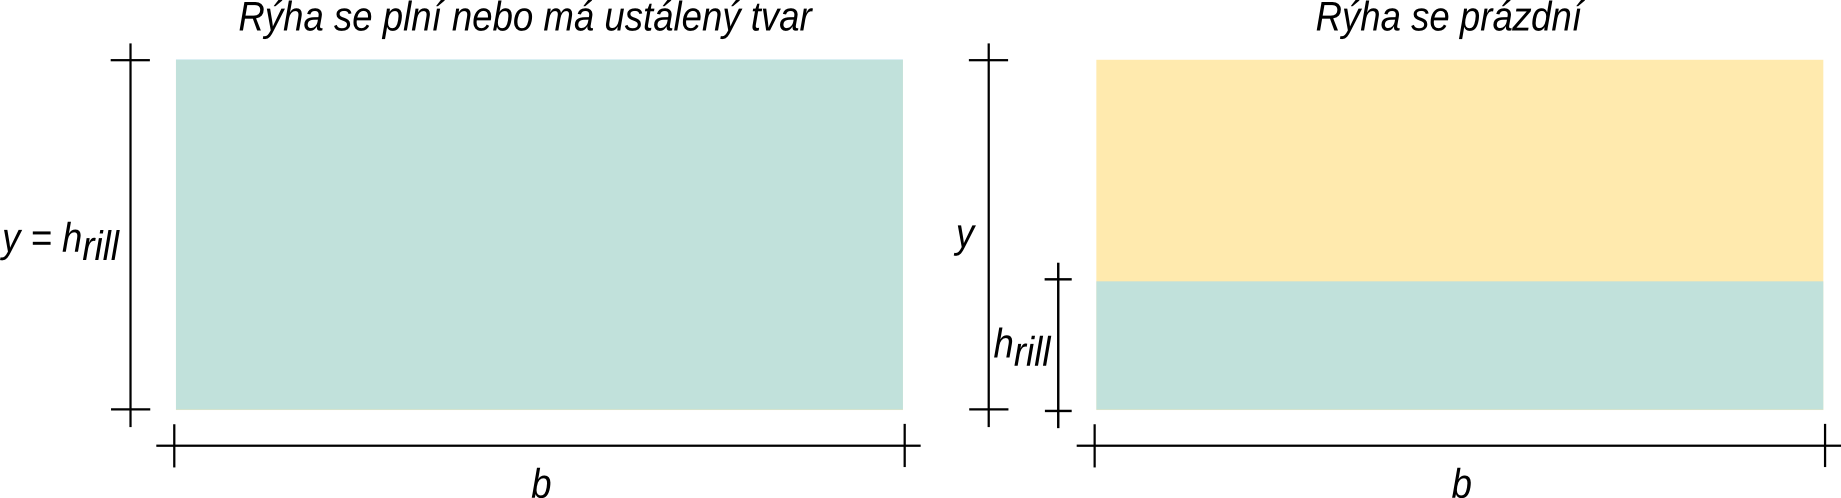
\includegraphics[width=0.9\textwidth]{./img/rill_schema.png}
    \caption{Tvar rýny a výška vodní hladiny při plnění rýny či ustálení proudění (napravo), tvar rýny při jejím prázdnění (nalevo)}
    \label{fig:rill_schema}
  \end{figure}
% 
%   
  $$ 
    \acs{Rrill} = \frac{\acs{A}}{\acs{O}} = \dfrac{\acs{hrill} \acs{brill}}{\acs{brill}+2\acs{hrill}} = \dfrac{\acs{brill}^{2} \acs{rratio}}{\acs{brill}(\acs{rratio}+2)}
  $$
  \begin{tabular}{rrl}
    kde \jj{brill}{,}
        \jj{O}{\ a}
        \jj{rratio}{.}
  \end{tabular}
  
  
%   Poměr šířky a výšky je v programu stanoven v současné době pevně, ale jako parametr, který je možné v případě potřeby změnit. Objem rýhy je stanoven podle rovnice \ref{Vrill}.

%   \item V případě poklesu objemu vody v rýze si rýha zachovává svůj maximální tvar.
\end{enumerate}


% Pro výpočet průtoku v rýze \acs{qrill} je pak možné využít Chézyho rovnici v manningově tvaru:.


\paragraph{Celková bilance}
Pokud dojde k vzniku rýh, přičtou se do celkové bilance~\ref{eq:bilancnirce} další dva členy vyjadřující přítok a odtok v rýhách. Rovnice~\ref{eq:bilancnirce} vypadá následovně

\begin{equation} 
\acs{hsur}_{i,t} = \acs{hsur}_{i,t-1} + \acs{dT}\left(\acs{es}_{i,t} + \sum_j^m \acs{oin}_{j,t-1} - \acs{inf}_{i,t} - \acs{oout}_{i,t-1}  + \sum_k^n \acs{oinrill}_{k,t-1} - \acs{ooutrill}_{i,t-1} \right),
\label{eq:bilancnircerill}
\end{equation}
  \begin{tabular}{rrl}
    kde \jj{oinrill}{\ a}
        \jj{ooutrill}{.}
        & $n$ & jsou buňky, odkud vtéká voda z rýh do buňky $i$.
  \end{tabular}\\
 $n$ může být prázdná množina pokud není překročena kritická výška nebo no může rovnat $m$ z rovnice~\ref{eq:bilancnirce} pokud je použit odtokový algoritmus \acs{D8} a na všech sousedních buňkách buňky $i$ je překročena kritická výška hladiny. 



\paragraph{Rýhový odtok \acs{oinrill}, \acs{ooutrill}}

Výška odtoku (resp. vtoku) z rýhy do dané výpočetní buňky je vypočtena za základě Chézyho rovnice~\ref{eq:qrill} takto:
$$
  \acs{oinrill} (resp.\ \acs{ooutrill}) = \frac{\acs{qrill}}{\acs{brill}\acs{lrill}}
$$
\begin{tabular}{rrl}
  kde \jj{lrill}{.}
\end{tabular}


% Množství odtoku \acs{Orill} za \acs{dT} je pak možné stanovit podle vztahu:
% \begin{eqnarray}
% O_{rill_{i,t}} [m^{3}] = \Delta t q_{sur}
% \end{eqnarray}
% 
% Tvar bilanční rovnice \ref{bilancnirce} při zavedení odtoku v rýhách pak přechází na tvar:
% \begin{eqnarray}
%   H_{i,j,t} = H_{i,j,t-1} + ES_{i,j,t} + \sum\limits_{(i,j)\in M} O_{M_{t-1}} - O_{i,j,t} - I_{nf_{i,j,t}} \label{eq:bilancenew}
% \end{eqnarray}
% \begin{equation*}
%  M = \{ (k,l) | i-1 \leq k \leq i+1 ; j-1 \leq l \leq j+1 \}
% \end{equation*}



% \textit{kde $ O_{M} $ obecně znamená jak přítok plošný, tak soustředěný v rýhách, $ O $ celkový odtok, který se podle konkrétního stavu dělí na plošný a soustředěný}





\paragraph{Poznámka nebo to dát do diskuse k článku} 
\begin{itemize}
\item Výsledný tvar blíží Maningově rovnici
\begin{eqnarray}
Q =\frac A {1}{n} R_{h}^{2/3} S^{1/2}
\end{eqnarray}
\item Přesněji pro tvar této rovnice pro plošný odtok, kdy se předpokládá proudění vody  o malé hloubce a tvar koryta je nahrazen jeho šířkou. Rovnice má pak tvar:
\begin{eqnarray}
Q =\frac {1}{n} h^{2/3} S^{1/2}
\end{eqnarray}
\item Že může být jiná rce infiltrace.
\item tvar rýhy - výzkum funkce?
\item jen jedna přímá rýha
\end{itemize}

%newb = math.sqrt(V/(rillRatio*l)) #KAvka, tohl eje divně
\subsubsection{Odtok hydrografickou sítí} \label{sec:tokyodtok}
\textbf{tohle není vůbec napsané}

kapitola nenese záměrně název vodní toky. SMODERP je zamýšlen také jako nástroj pro navrhování opatření v ploše povodí. Cílem je simulovat a navrhovat odtoky i v dočasné hydrografické síti, která je tvořena přirozeným nebo častěji umělým přerušením přirozené odtokové dráhy. Nejčastěji se jedná o příkopy a průlehy které mají odváděcí a často erozní funkci. 
Všechny prvky (síť vodních toků, přkopy, průlehy, atp.) jsou zadávány v rámci jednoho shapefile. Každý jednotlivý úsek je zadán jako konkrétní polygon (feature). Výpočetně model pracuje v rastrové síti, ale v případě, že se na daném elemetu vyskytuje tok, je přiteklá voda dále odváděna tímto tokem ve směru toku bez ohledu na směr odtoku modelu terénu.

Proudění v těchto otevřených korytech je řešeno Mannigovou rovnicí ve tvaru:

\textbf{překotrovat rci}
\begin{equation}
    \acs{qstream} = \acs{A} \frac{1}{\acs{n}} \acs{Rsheet}^{2/3} \acs{I}^{1/2}  ,
    \label{eq:qtok}
\end{equation}

%\begin{tabular}{stream}
 %   kde \jj{qstream}{,}
  %      \jj{vstream}{,}
   %     \jj{A}{,}
    %    \jj{n}{\ a}
     %   \jj{Rstream}{.}
%\end{tabular


Pro vlastní výpočet je třeba zadat typ a příčný profil daného prvku. Délka úseku je převzata z vlastností polygonu. Protože je model určen pro malá povodí jsou v modelu předpokládány pouze základní příčné profily (trojúhelník, obdélník, lichoběžník, parabola). 
Zadávání příčných profilů není přímo součástí shapefile, ale pro ulehčení jsou parametry zadávány jako samostatná tabulka. V případě, že jsou některé charakteristiky shodné, je tak možné jim přiřadit shodné atributy z tabulky.
V rámci zjednodušení výpočtu jsou zadávány profily parametricky. Zjednodušený výpočetní model neuvažuje rozlivy z koryta zpět do buněk odtoku. Jednotlivé prvky narůstají podle zvolených parametrů, tak aby veškerá voda zůstala v korytě.
přehled parametrů je uveden v následující tabulce

\textbf{vlžit tabuklu peka}

cislo	smoderp	tvar	b	m	drsnost	Q365	pozn
0	0	1.0	0.3	1.0	0.03	0.0	default
1	obdelnik1	0.0	0.2	0.0	0.035	0.0
2	lichobeznik1	1.0	0.2	2.0	0.035	0.0
3	trojuhelnik1	2.0	0	2.0	0.03	0.0
4	parabola1	3	0.7	0.0	0.03	0.0	b..sirkahladina




kde:
\begin{itemize}
\item \textbf{b} - šířka profilu ve dně (u trojúhelníku se rovná nule)
\item \textbf{m} - poměr sklonu svahů (pro obdélník je roven nule)
\item \textbf{drsnost} - Maninngova drsnost v daném korytě.
\item \textbf{Q365} - základní odtok. V případě dočasných prvků jako jsou příkopy je tato hodnota rovna nule, v případě vodních toků se jedná o základní odtok.-
\item \textbf{poznámky} - jedná se o volitelnou položku, do výpočtu se nijak nepropaguje
\end{itemize}

Tímto způsobem jsou zadávány
\textbf{sem dát obrázek těch profilů}


\textbf{doplnit text jak probíhá vlastní výpočet} - tzn jak na sebe navazují jednotivé úseky . a dát semka asi i nějaké  obrázky, jak to funguje. Je to v nějaké DP tuším (to najdu PK)







\newpage
\section{Výsledky}
%!TEX ROOT = ../mainCZ.tex
%\input{./1_text/3_mat_a_met/2}

Úvodní část je věnována historickému pozadí a vývoji modelu SMODERP. Odvození parametrů o kterých se hovoří v kapitole \ref{SM_hist} jsou podrobně popsány v kapitole \ref{Exp_mer}. Použité fyzikální vztahy jsou popsány v kapitole \ref{modelovani}. SOučasná verze modelu z hlediska zpracování vstupních dat, výpočtu a uváděných výstupů je pak v kapitole \ref{vypocet}.


\setcounter{section}{0}
\section{Porovnání metod 1D a 2D} \label{porovnani1D2D}
\setcounter{section}{0}
\section{Porovnání metod 1D a 2D} \label{porovnani1D2D}


1D and 2D approaches which are subject to comparison were designated by a hydrograph and runoff volume in the breach profile. The respective comparison was carried out on two locations in the Czech Republic (Hořanský stream and Býkovický catchment). A system of erosion control measures was implemented in this area. The size of the given area being subject to this research is 1.5 $ km^{2} $. For 1D model are the individual agricultural plots were distinguished by 12 different profiles.

\begin{figure}[ht!]
\centering
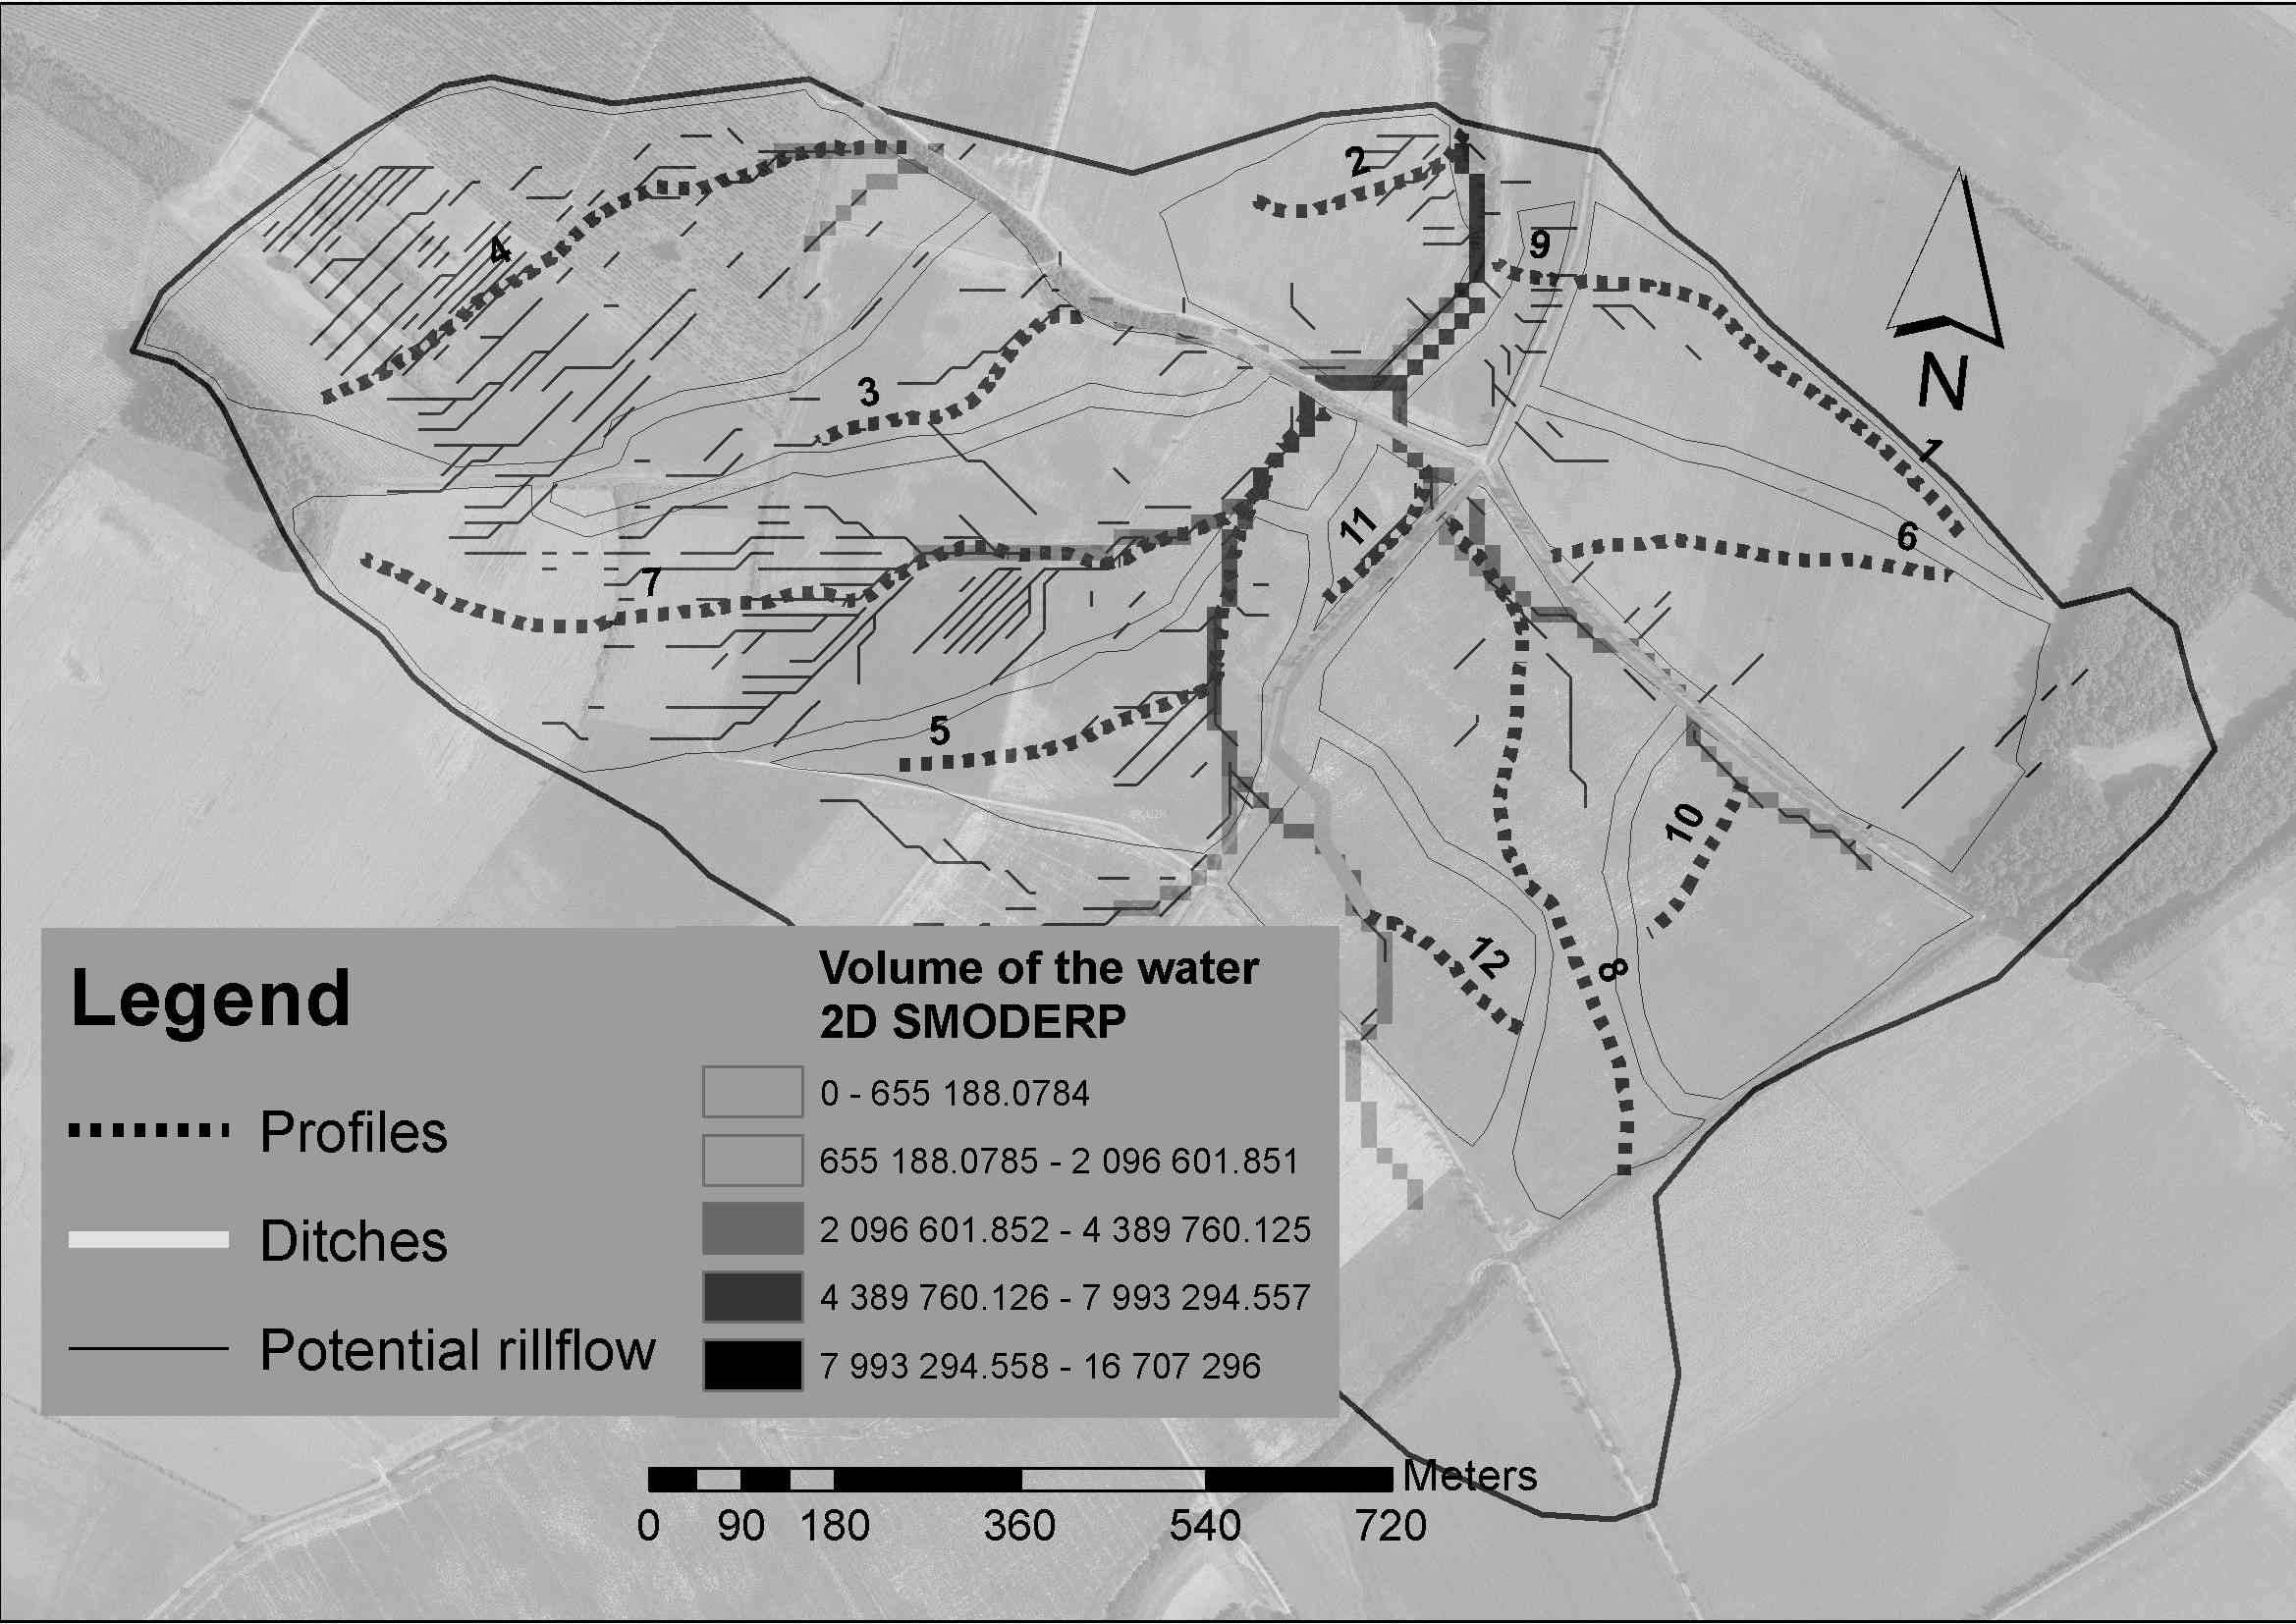
\includegraphics[width=0.8\textwidth]{img/horany_print3.jpg}
\caption{Profiles and runof concetration - Horany}
\label{fig:horany}
\end{figure}\FloatBarrier

\begin{figure}[ht!]
\renewcommand{\figurename}{Graf}
\centering
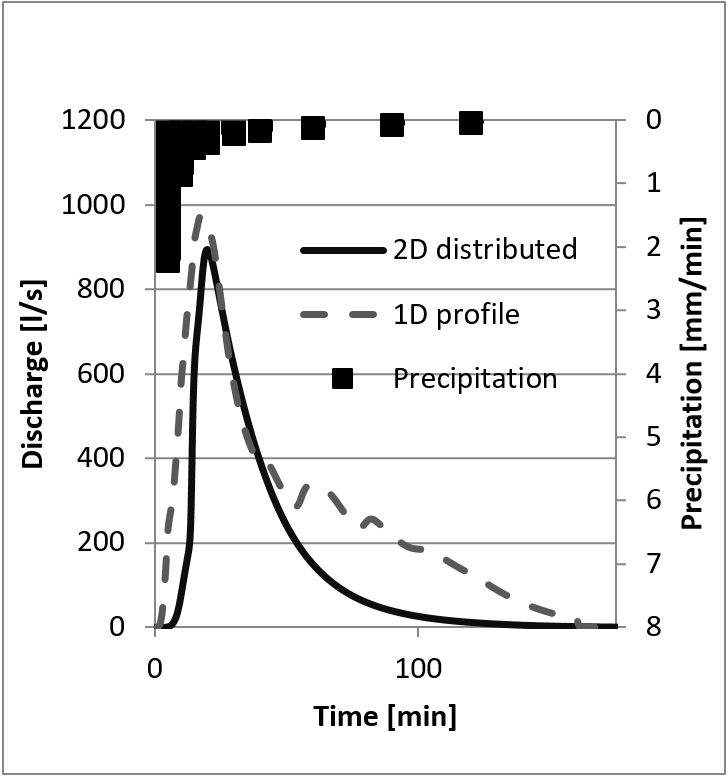
\includegraphics[width=0.8\textwidth]{graph/1D2Dhorany.png}
\caption{Hydrographs 1D and 2D Smoderp - Horany study area}
\label{graf:graf_1}
\end{figure}\FloatBarrier

The second location is formed by the independent agricultural plot situated in the Býkovický potok basin (Benešov u Prahy) with a morphologically distinctive lane of concentration runoff. Experimental measurements of erosion processes were carried out on the given plot for a considerable period of time. It is thus possible to compare the final results for the appropriate model with measured values. Six characteristic profiles were created on the given plot (size of ten acres). This number exceeds considerably the amount of profiles which were necessary for the description of the given small area. The number of profiles was appointed in order to make comparisons between 1D and 2D approaches, as well as from the reasons explaining the influence of a large number of profiles on the final characteristics. Standardized field erosion plots were installed and situated on a farmer plot in the surveyed area for monitoring the overland flow and sediment transport. The resulting cooperation between the 1D and 2D approaches was executed during the real rainstorm with measured surface runoff.

\begin{figure}[ht!]
\centering
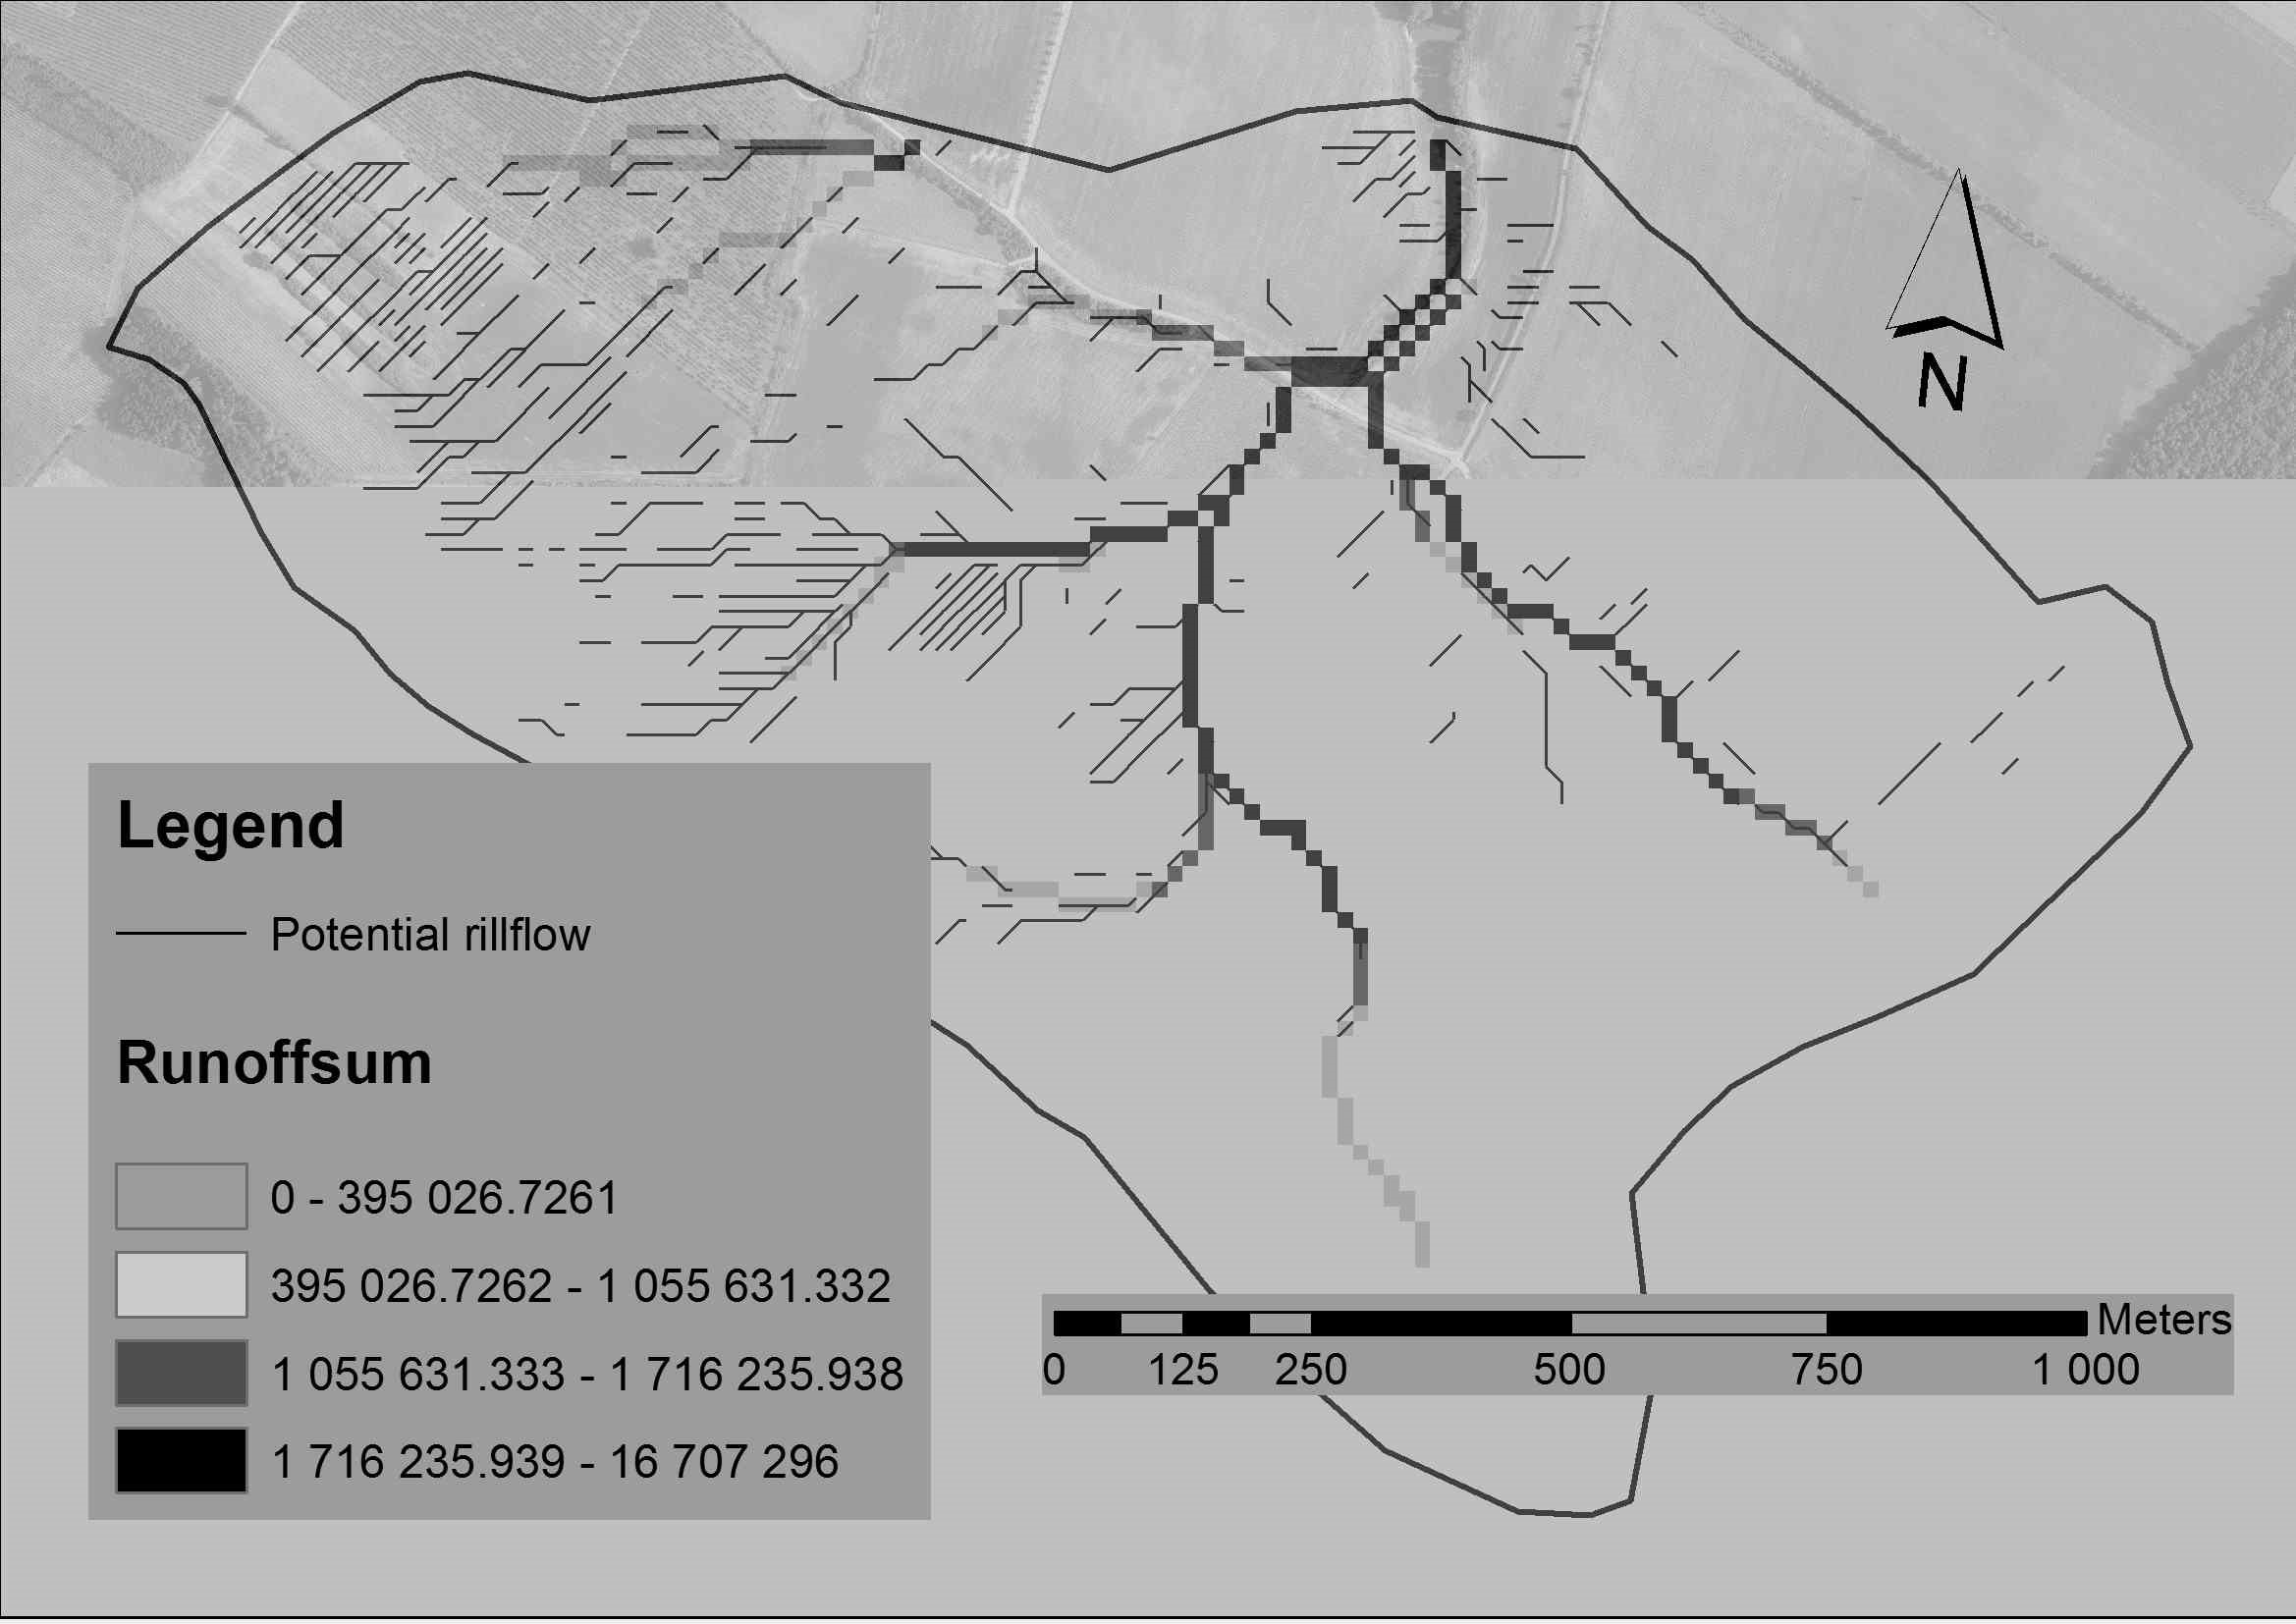
\includegraphics[width=0.8\textwidth]{img/byk.jpg}
\caption{Profiles and runof concetration - Bykovicky catchment }
\label{fig:horany}
\end{figure}\FloatBarrier

\begin{figure}[ht!]
\renewcommand{\figurename}{Graf}
\centering
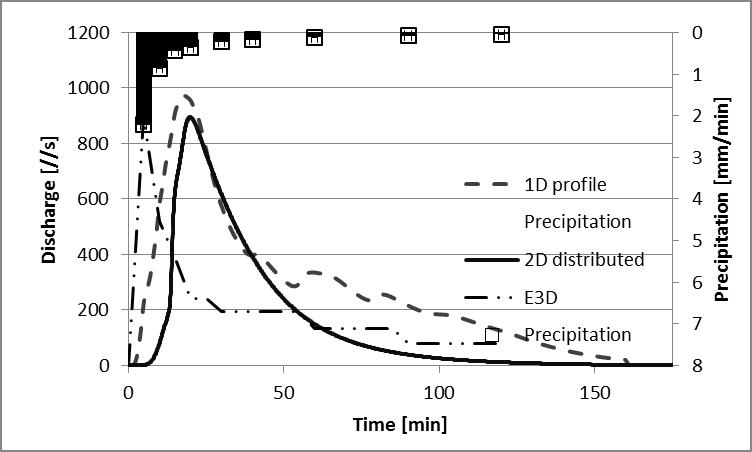
\includegraphics[width=0.8\textwidth]{graph/1D2DByk.jpg}
\caption{Hydrographs 1D and 2D Smoderp - Bykovicky catchment}
\label{graf:graf_1}
\end{figure}\FloatBarrier

The results based on hydrograph measurements taken from individual profiles in both locations were progressively added to the breach profile (outlet). In order to compare the discharge process, the values of surface level, discharge and a cell of the breach profile were extracted in the 2D model version for testing. The implementation of this process is enabled in the development environment of the particular model.

%\clearpage
%\newpage\null\thispagestyle{empty}\newpage


\newpage
%!TEX ROOT = ../../main.tex
%\chapter*{}
\section{Seznam použitých zdrojů}
\bibliographystyle{csplainnat}
% \addcontentsline{toc}{section}{Literatura}

\lhead[\sl{Literatura}]{}
\rhead[]{\sl{Literatura}}
%\bibliography{bib/erosion,bib/kavka,bib/models}
\bibliography{bib/bib}

\clearpage



\end{document}

